\documentclass{article}

\usepackage{float}
\usepackage{graphicx}
\usepackage[dutch]{babel}

\usepackage{hyperref}
\hypersetup{
    colorlinks=true,
    linkcolor=black,
    filecolor=blue,      
    urlcolor=blue,
    pdfpagemode=FullScreen,
}

\title{Slicen en plannen}
\author{Martijn Voorwinden 1776622}
\date{10-11-2022}

\newcommand{\us}[8]{
    \maketitle
    \subsection*{Inleiding}
    #1
    \subsection*{Criteria}
    \begin{itemize}
        \item Kwalitatief product maken.
        \item Planning - een planning opstellen.
        \item Verantwoorden van (noodzakelijke aanpassingen in) planning.
    \end{itemize}
    \subsection*{User Story}
    % ss van story in backlog
    \textbf{#2}
    #3
    \subsubsection*{Taken}
    % itemize
    #4
    \subsubsection*{Acceptatiecriteria}
    % itemize
    #5
    \subsubsection*{Definition of Done (DoD)}
    % itemize
    #6
    \subsubsection*{Estimate}
    #7
    \subsubsection*{Realisatie}
    #8
    \\ \newline \href{https://github.com/MartijnCBV/INNO/tree/master}{Product tot nu toe.}
}

\begin{document}
    \us
    {
        Voor provincie Utrecht moet er een datacatalogus gemaakt worden om de medewerkers makkelijker toegang te geven tot de verschillende databronnen in de verschillende afdelingen van de provincie.
        Dit is nodig om te zorgen dat er geen dubbele datasets worden aangeschaft en om de zoektijd naar relevante datasets te verkleinen.
        Mijn rol binnen dit project is developer.
    }
    {
        Als gebruiker wil ik relevante datasets of informatieproducten \\ aangeboden krijgen wanneer ik op trefwoorden zoek zodat ik voor mij benodigde informatie kan binnenhalen.
    }
    {
        \begin{figure}[H]
            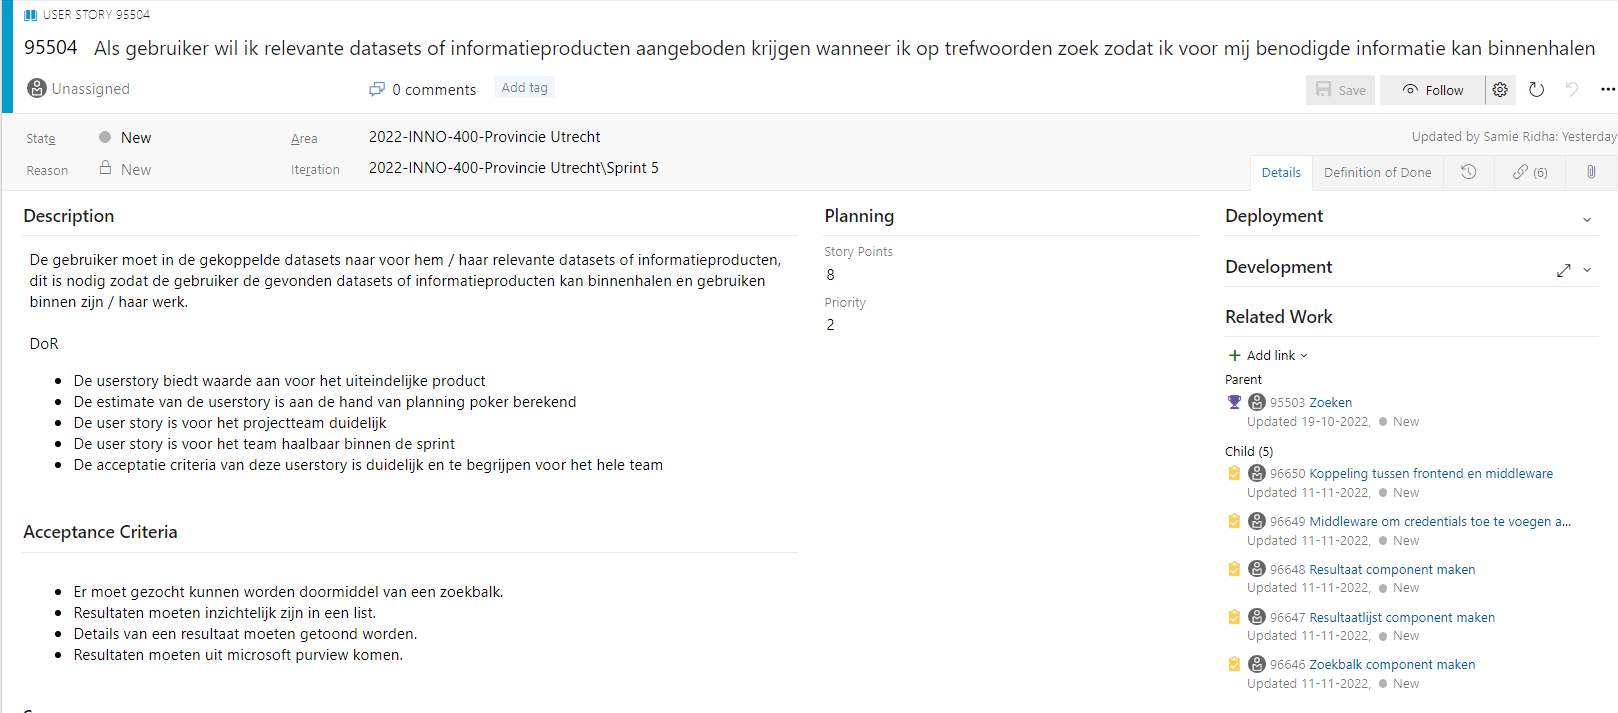
\includegraphics[width=\textwidth,height=\textheight,keepaspectratio]{us_01.png}
            \caption{\href{https://dev.azure.com/HU-HBO-ICT/2022-INNO-400-Provincie\%20Utrecht/_backlogs/backlog/2022-INNO-400-Provincie\%20Utrecht\%20Team/Epics/?workitem=9550}{De user story in devops.}}
            \label{fig:us_01}
        \end{figure}
        \noindent De gebruiker moet in de gekoppelde datasets naar voor hem / haar relevante datasets of informatieproducten,
        dit is nodig zodat de gebruiker de gevonden datasets of informatieproducten kan binnenhalen en gebruiken binnen zijn / haar werk.
    }
    {
        \begin{itemize}
            \item Zoekbalk component maken.
            \item Resultaatlijst component maken.
            \item Resultaatcomponent maken.
            \item Middleware om credentials toe te voegen aan request maken.
            \item Koppeling tussen frontend en middleware.
        \end{itemize}
    }
    {
        \begin{itemize}
            \item Er moet gezocht kunnen worden doormiddel van een zoekbalk.
            \item Resultaten moeten inzichtelijk zijn in een lijst.
            \item Details van een resultaat moeten getoond worden.
            \item Resultaten moeten uit microsoft purview komen.
        \end{itemize}
    }
    {
        \begin{itemize}
            \item De userstory is grondig getest met behulp van verschillende test\\ methodieken.
            \item De userstory heeft een peer review gekregen van tenminste een collega.
            \item De acceptatie criteria komt overeen met de userstory.
            \item De product owner gaat akkoord met het resultaat van de userstory.
        \end{itemize}
        %\begin{itemize}
        %    \item Er is een applicatie ontwikkeld die volgens de elm architectuur werkt.
        %    \item Elm-review geeft geen errors
        %    \item De applicatie voldoet aan de elm style guide
        %    \item De applicatie is opgedeeld in modules
        %\end{itemize}
    }
    {
        We zijn tot een estimate gekomen van 8 / 10 storypoints, 
        dit omdat het, het hoofdcomponent van de applicatie is en omdat er meerdere verschillende stukken van de applicatie geraakt worden.
    }
    {
        De user story is een aantal keer verplaatst vanwege een gebrek aan toegang tot purview,
        hierdoor kon er nog niet veel gedaan worden. \\ \newline
        Nog niet volledig geraliseerd.
    }
\end{document}